\documentclass[letterpaper, 10 pt, conference]{ieeeconf}  % Comment this line out if you need a4paper

%\documentclass[a4paper, 10pt, conference]{ieeeconf}      % Use this line for a4 paper

%\IEEEoverridecommandlockouts                              % This command is only needed if 
                                                          % you want to use the \thanks command

%\overrideIEEEmargins                                      % Needed to meet printer requirements.

% See the \addtolength command later in the file to balance the column lengths
% on the last page of the document

% The following packages can be found on http:\\www.ctan.org
\usepackage{graphics} % for pdf, bitmapped graphics files
\usepackage{epsfig} % for postscript graphics files
\usepackage{graphicx}
\usepackage{mathptmx} % assumes new font selection scheme installed
\usepackage{times} % assumes new font selection scheme installed
\usepackage{mathtools} % assumes amsmath package installed
\usepackage{amssymb}  % assumes amsmath package installed
\usepackage{tikz}
\usepackage{tabulary}
\newcommand{\hvec}{\overset{\rightharpoonup}}
\newcommand{\argmin}{\arg\!\min}
\newcommand{\norm}[1]{\left\lVert#1\right\rVert}
\newcommand{\quotes}[1]{``#1''}
\usetikzlibrary{calc,positioning, fit, arrows}
%\usepackage{biber}

%for citing webcites
\usepackage{cite}
\usepackage{url}

\makeatletter
\newenvironment{tablehere}
  {\def\@captype{table}}
  {}

\newenvironment{figurehere}
  {\def\@captype{figure}}
  {}
\makeatother

\newcommand{\vect}[1]{\ensuremath{\mathbf{#1}}}
\newcommand{\mat}[1]{\ensuremath{\mathbf{#1}}}
\newcommand{\transpose}{\ensuremath{\mathsf{T}}}
\newcommand{\of}[1]{\ensuremath{\left(#1\right)}}

\title{\LARGE \bf
Multi-dimensional Optimization of Gasoline-fueled Variable Pitch Multirotor Aircraft
}


\author{Dallin Briggs, Gary Ellingson% <-this % stops a space
%\thanks{$^{1}$James Jackson is a MS student in the Department of Mechanical Engineering, Brigham Young University
%        {\tt\small jamesjackson@byu.edu}}%
%\thanks{$^{2}$Gary Ellingson is a MS student in the Department of Mechanical Engineering, Brigham Young University
%        {\tt\small gary.ellingson@byu.edu}}%
}


\begin{document}



\maketitle
\thispagestyle{empty}
\pagestyle{empty}


%%%%%%%%%%%%%%%%%%%%%%%%%%%%%%%%%%%%%%%%%%%%%%%%%%%%%%%%%%%%%%%%%%%%%%%%%%%%%%%%
\begin{abstract}

Currently, there are numerous multirotor unmanned aerial vehicles (UAVs) that are available to commercial operators and to consumers that are capable of lifting small payloads for an endurance of approximately 30 minutes or less. While these current multirotors are good for short endurance missions, there are few options for larger, higher payload capacity multirotors that are able to maintain flight for longer than an hour. This paper describes the optimization process used to develop a multirotor platform that maximizes the flight time of a gasoline-fueled multirotor UAV by varying several design variables related to the power required and the aerodynamics of the model.

\end{abstract}


%%%%%%%%%%%%%%%%%%%%%%%%%%%%%%%%%%%%%%%%%%%%%%%%%%%%%%%%%%%%%%%%%%%%%%%%%%%%%%%%
\section{INTRODUCTION}

The creation of a multirotor aircaft capable of both carrying a relatively large payload and flying for a long duration would be very desirable for many applications.

Designing a gas powered multirotor aircraft requires several design decisions. When considering the total flight time of a the aircraft, foremost of these design decisions are the choices of rotor, engine and gas tank size.  These design decisions along with several other aircraft parameters all have trade-offs that makes it difficult for a designer to simultaneously consider which trade-offs will allow for the longest flight time and/or greatest payload capacity. 

This paper presents analysis and optimization methods for designing a gas powered multirotor aircraft.  The analysis focuses on modeling the engine and aerodynamic components with a limited consideration of aircraft structure.  These analyses are then used within multi-dimensional optimization to produce a vehicle design capable of long duration flight. 

%%%%%%%%%%%%%%%%%%%%%%%%%%%%%%%%%%%%%%%%%%%%%%%%%%%%%%%%%%%%%%%%%%%%%%%%%%%%%%%
\section{BACKGROUND}

Multirotor aircraft are useful for a variety of applications.  Because multirotors can fly vertically, they do not require landing strips.  They can carry sensor equipment for scientific or surveillance purposes. Multirotor use in package delivery is being studied by several large companies such as Google, Amazon and DHL \cite{Amazon2014}.   

Incorporating a gas powered engine into a multirotor requires more then just exchanging the electric motors and batteries for an engine and a gas tank, respectively. The control of such a vehicle would also fundamentally change.  Electric multirotors are controlled by varying propeller rotational speed to produce varying thrust and torque, which in turn controls the attitude of the aircraft. Gas engines lack the ability to vary speed quickly enough to control the attitude of a multirotor aircraft. This means a fixed speed and variable pitch propeller is better suited for a gas powered vehicle.

Variable pitch mulitrotor aircraft are not as common as variable speed multirotors but they have been explored to some degree. Control of variable pitch multirotor aircraft was studied by Cutler \cite{Cutler2012}. There is a small, electric variable pitch quadcopter commercially available \cite{stingray2016} for performing stunts and inverted maneuvers.  There are also several hobbyist attempts at gas powered variable pitch quad-rotor (quads) \cite{diy2016}, \cite{hackaday2016}. In our knowledge there has been no attempt to use a gas powered variable pitch quad to maximize the flight time for carrying a relatively large payload for commercial applications. 

There are many commercially available components that could be used to create a gas powered multirotor, including engines \cite{da2016} and variable pitch helicopter propellers \cite{align2016}. However, a gas powered multirotor would required a custom frame for mounting the engine and supplying power from the engine to the individual rotors.

FAA requirements \cite{faa2016} specify that model aircraft and UAVs of any sort must weigh less then 55 lbs (25 kg). UAVs or model aircraft weighing more than 55 lbs require special airworthiness certificates and are much more heavily regulated.

\section{MOTIVATION}

Nearly all commercial and consumer multirotor UAVs are powered by lithium-polymer batteries because of their relatively high energy capacity to weight ratios. Although these batteries are very useful and reliable, they still offer much lower specific energy ratios than that of liquid fuels such as gasoline. The average specific energy for lithium-polymer batteries is approximately 0.95 MJ/kg \cite{Battuni2016}, where gasoline is 46.4 MJ/kg \cite{energyed2016}. This means that a gasoline-fueled multirotor can potentially fly much longer than a battery powered vehicle because it can carry more energy.

\begin{figurehere}
	\begin{center}
		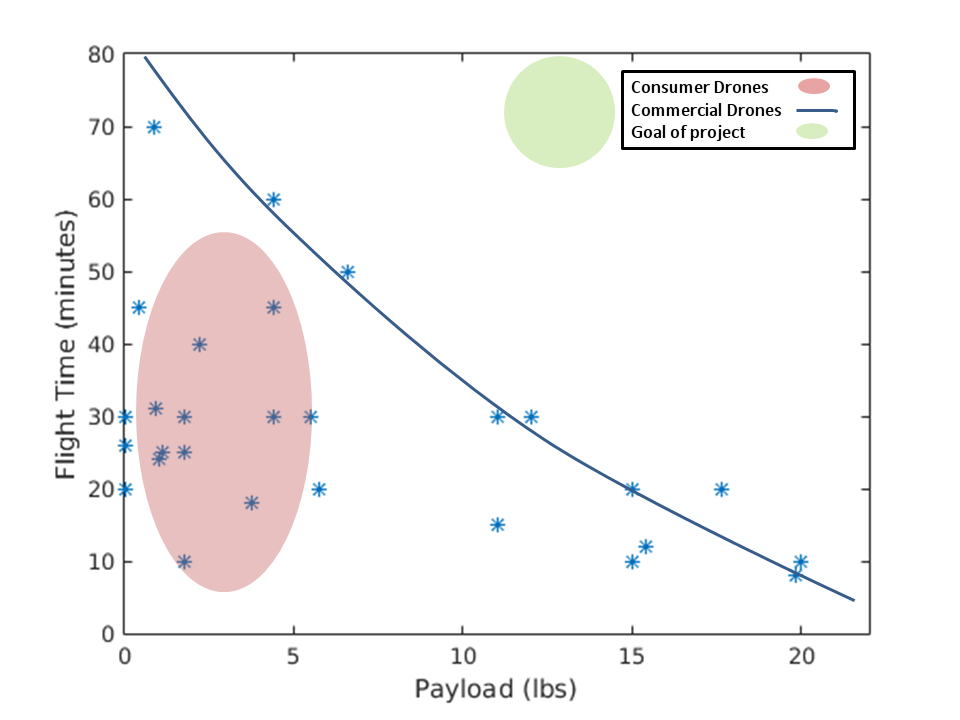
\includegraphics[width=.5\textwidth]{current_capabilities.png}
		\caption{\textit{Graphic showing capabilities of current platforms and the goal of this project. The data points shown are specifications given by manufacturers of popular commercial and consumer UAVs and is collected from \cite{drones2016}.}} 
		\label{fig:current_cap}
	\end{center}
\end{figurehere}

The goal of this project is to expand the flight envelope of multirotor aircraft.  Figure~\ref{fig:current_cap} demonstrates the current capabilities of consumer and commercial multirotors and depicts the goal of this project.  We believe that a multirotor that could carry larger payloads for longer periods of time would greatly expand the type and number of applications for these vehicles. A multirotor with this capability would fundamentally change the way multirotors are used in commercial applications. 

%%%%%%%%%%%%%%%%%%%%%%%%%%%%%%%%%%%%%%%%%%%%%%%%%%%%%%%%%%%%%%%%%%%%%%%%%%%%%%%%%%
\section{METHODS}

Because the quad is going to be built using commercially available off-the-shelf components, the optimization must be closely based on a realistic model. Therefore, the analysis must either be based on observations from available hardware or attempt to analyze the hardware in its available configurations.  The following sections present some surrogate models for approximating engine parameters as well as an aerodynamic analysis of common variable pitch RC propellers. 

\subsection{Engine} 

The designer essentially can only choose the size of engine when choosing a power plant. All the other data about the engine (mass, maximum power, etc.) have to be functions of displacement size.  Data was collected for popular two stroke RC aircraft engines from several sources to produce the models for other unknown parameters. One source for engine data was Desert Aircraft \cite{da2016}.  Figure~\ref{fig:mass} shows the collected data for engine size and mass.  We performed a linear least squares best fit to produce a model for use in our analysis.

\begin{figure}
	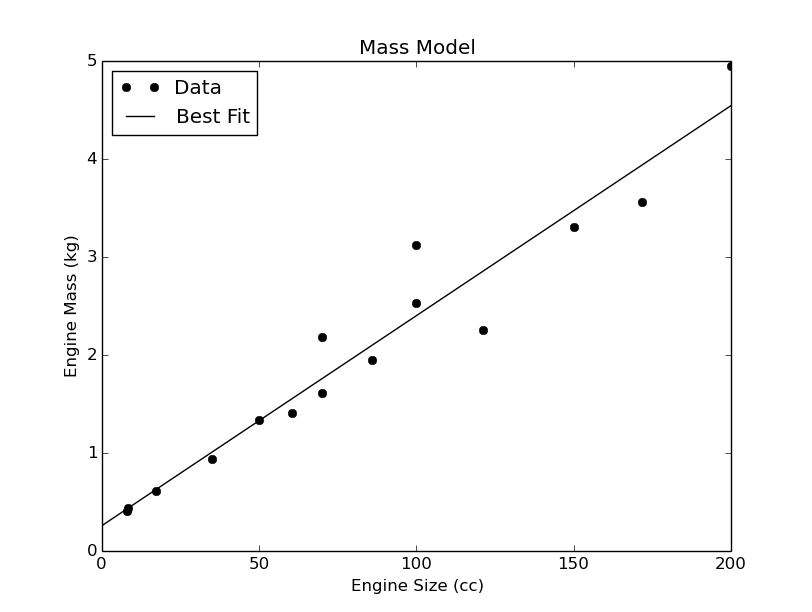
\includegraphics[width=0.5\textwidth]{mass.png}
	\caption{The empirical data based surrogate model of engine mass as a function of displacement size. Data from desertaircraft.com \cite{da2016}. $\ y = ax + b \quad a = 0.02145 \quad b = 0.25412$}
		\label{fig:mass}
\end{figure}

Data was also used to produce a model of the power output of the engine as a function of size. Figure~\ref{fig:power} shows the collected data for engine size and power.  Again, we initially used a linear least squares fit to the data as well as compared our fit to data produced by Barnard Microsystems \cite{barnardmiro2016}. However, both models were inadequate for our analysis because they contain a non-zero y-intercept.  A non-zero y-intercept would allow an infinitely small engine to produce power and thus would allow the aircraft to fly infinitely. To correct for this issue, we applied a quadratic fit to the data and forced it to intercept through the origin.

\begin{figure}
	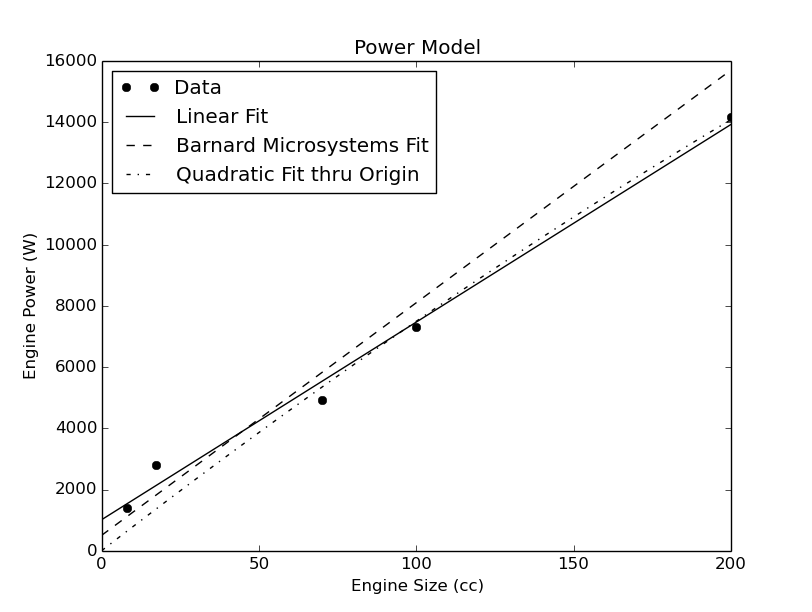
\includegraphics[width=0.5\textwidth]{max_power.png}
	\caption{Empirical based surrogate model of engine maximum power as a function of displacement size. Notice the linear models have a non-zero y-intercept but the quadratic fit goes through the origin. Data from desertaircraft.com \cite{da2016} and barnardmicrosystems.com \cite{barnardmiro2016} $\ y = ax^2 + bx \quad a = -0.04548 \quad b = 79.504$}
		\label{fig:power}
\end{figure}


The engine efficiency was not modeled for this project and was assumed as a constant parameter.  Throughout the analysis, the shaft output power of the engine was 15\% of the power consumed from the fuel.  

\subsection{Aerodynamics}

Much of the work done in the methodology of optimizing flight time was to find adequate models for the thrust, torque, and power required from the main rotor disks. Since each rotor will be designed using small-scale helicopter components that consist of variable-pitch rotors that have no twist, a simplified helicopter rotor aerodynamic model should be sufficient for these calculations. 

Many of the existing aerodynamic models used in the aerospace industry to represent helicopter rotors are extremely complex and require specialized software tools (many of which are proprietary). High fidelity aerodynamic models generally require lots of computational power; so in order to focus on optimization methods, rather than the complex aerodynamic interactions of the system, several simplifications were made in analyzing the inflow angle and the down-wind air interactions of the propeller. Also, the model used assumes the multirotor is in hover, since that seems to be the primary use condition of multirotor aircraft.

Combined differential blade element and momentum theory for nonuniform inflow was used to calculate the thrust and the torque differentially across each rotor blade \cite{bramwell2001bramwell}. Using blade element theory, the differential thrust is given by

\begin{equation}
	dT_{prod} = \frac{1}{2} \rho a \Omega^2 r^2 (\theta - \phi) c \  dr,
	\label{thrust_eqn}
\end{equation}

where $\rho$ is the air density, \textit{a} is the lift-curve slope for the blade airfoil, $\Omega$ is the angular velocity of the rotors, \textit{r} is the radius of the annulus of the rotor being differentiated, $\theta$ is the blade pitch angle measured from the horizontal plane formed by the rotational disc of rotor blades, \textit{c} is the chord of the rotor, and $\phi = \tan^{-1}(U_p/U_T) $ is the inflow angle at the blade element. $U_P$ and $U_T$ are the components of air velocity relative to blade element perpendicular and tangential to the plane of rotation, respectively. The total thrust on each rotor is calculated by integrating equation \ref{thrust_eqn} across the rotor radius, \textit{R}. The total thrust for the multirotor, $T_{prod}$ can then be calculated by multiplying the rotor thrust by the number of \textit{N} rotors. 

The differential torque for each rotor blade is given by

\begin{equation}
	dQ_{req} = \frac{1}{2} \rho \Omega^2 r^3 c (\delta + \phi C_L) \ dr,
	\label{torque_eqn}
\end{equation}

where $\delta$ is the local blade drag coefficient, and $C_L$ is the lift coefficient. The total torque for the multirotor , $Q_{req}$, can be found using the same method for calculating the total thrust. 

The differential power produced by each rotor is then given by 

\begin{equation}
	dP_{req} = dQ\Omega,
	\label{power_eqn}
\end{equation}

and the total power required by the rotors, $P_{req}$, can be calculated using the same method as total thrust and torque \cite{venkatesan2014fundamentals}. 

Equations \ref{thrust_eqn}, \ref{torque_eqn} and \ref{power_eqn} are used in the constraints, as discussed in the Optimization section. In practice, the thrust, torque, and power were integrated in a \textit{for loop} that divided each blade into 10 elements and then summed the differential values for each element. More divisions were made initially, but it greatly increased the computation time of the optimization algorithm and the results were approximately the same. 

Since the goal of this project is to optimize the flight time of a multirotor and then build it using existing remote controlled aircraft components, a NACA 0012 airfoil was used in the analysis for calculating the coefficient of lift, $C_L$, and the blade element drag coefficient, $\delta$. This airfoil approximately represents the airfoil of many commonly used remote control helicopters \cite{mettler2013identification}. Data points for this airfoil were generated using Xfoil, an aerodynamics tool developed by The Massachusetts Institute of Technology. This data was then fit with polynomials to approximately represent $C_L$ and $\delta$ across a range of the angles of attack, $\alpha$, continuously, where $\alpha = \theta - \phi$. 

Momentum theory allows for a relatively simple calculation of the inflow angle for each element of the blade. This calculation is an approximation, but it is sufficient for our low-fidelity model in designing the rotor system. The inflow angle is given by 

\begin{equation}
\phi^2 = (\frac{a\sigma}{8})(\theta-\phi),
\label{inflow_eqn}
\end{equation}

where 

\[ \sigma = \frac{bc}{\pi r} \]

is the blade solidity ratio based on local rotor radius, and \textit{b} is the number of blades in each rotor. 


\section{OPTIMIZATION}

Within the optimization there are two sets of design variables.  First, the design variables that influence the size of the vehicle: the rotor radius $R_{rot}$, the engine size $S_{eng}$, and the fuel capacity $f_{capacity}$.  Then, there are the design variables that are used to determine feasibility of the design: fuel burn rate $f_{rate}$, rotor pitch angle $\theta_{pitch}$, and propeller head speed $\omega_{rot}$. Number of blades per rotor and number of rotors were also initially treated as design variables. However, with the current aerodynamic model, the optimizer will create as many rotors with as many blades as possible to minimize the rotational speed required of each rotor to reduce the overall drag. Since adding more rotors would have un-modeled adverse affects on cost, complexity, and weight these variables are fixed as parameters in the analysis. Moving forward we will assume four sets of two blade rotors because this is a common configuration that would be reasonably simple to build.

%The flight time of the vehicle is only directly proportional to two of the design variables: the fuel capacity $C_{fuel}$ and the fuel burn rate $r_{fuel}$.  Once the fuel is all burned then the vehicle must land.  Through the constraints imposed on the optimization the flight time becomes indirectly a function of the rest of the design variables.

We now setup the formal optimization problem
\begin{equation}
	\begin{split}
		min. & \quad f\of{x} = -t_{flight}\of{x} \\
		w.r.t. & \quad x = [R_{rot}, S_{eng}, f_{capacity}, f_{rate}, \theta_{pitch}, \omega_{rot}]^T \\
		s.t. & \quad cons\of{x} \leq 0 
	\end{split}
	\label{eq:objective}
\end{equation}

where flight time was calculated by 
\[
	t_{flight} = K_{energy}\frac{f_{capacity}}{f_{rate}}.
\]
Without constraints, the solution to maximizing flight time would be trivial to calculate as well as impossible to construct. Therefore to optimize the system we must use constraints that ensure the quad is feasible and legal, according to the FAA \cite{faa2016}. The constraints are on the power produced by the engine ($P_{shaft}$), power required by the rotors ($P_{rot}$), thrust produced by the rotors ($T_{prod}$), total weight of the vehicle ($W_{total}$) and maximum power capabilities of the engine ($P_{max}$). To use the constraints correctly, the following relationships must hold:

\[
	\begin{split}
	P_{rot} & \leq P_{shaft} \\
	W_{total} & \leq T_{prod} \\ 
	P_{shaft} & \leq P_{max} \\
	W_{total} & \leq 55 lbs
	\end{split}
\]

The above aerodynamic model is used to calculate $P_{rot}$ and $T_{prod}$. $P_{shaft}$ is calculated from the fuel burn rate and engine efficiency. $W_{total}$ is the combined weight of the engine, vehicle frame, fuel, and payload. $P_max$ comes from the surrogate engine power model depicted in figure~\ref{fig:power}.

The design variables were scaled for input in to the optimizer. The optimizers we used were the Matlab's \textit{fmincon} function using interior-point algorithm and the Python \textit{pyoptsparse} package using SNOPT algorithum. Gradients were found using automatic-differentiation in Matlab and finite-differencing in Python. 

Our optimization algorithm found the maximum flight time given a payload, but another formulation would be to find the maximum payload given a specified flight time. This means we could create a Pareto frontier of this multi-objective optimization. However, to simplify we can create figure~\ref{fig:payload} by varying the payload parameter within our optimization (not a true Pareto frontier because payload was not specifically optimized). We then can further explore how the characteristics of a gas quad change as we optimize the flight time for different payloads. For example, figure~\ref{fig:eng_v_pl} shows how the optimal engine size changes as the payload parameter varies. 

\begin{figure}
	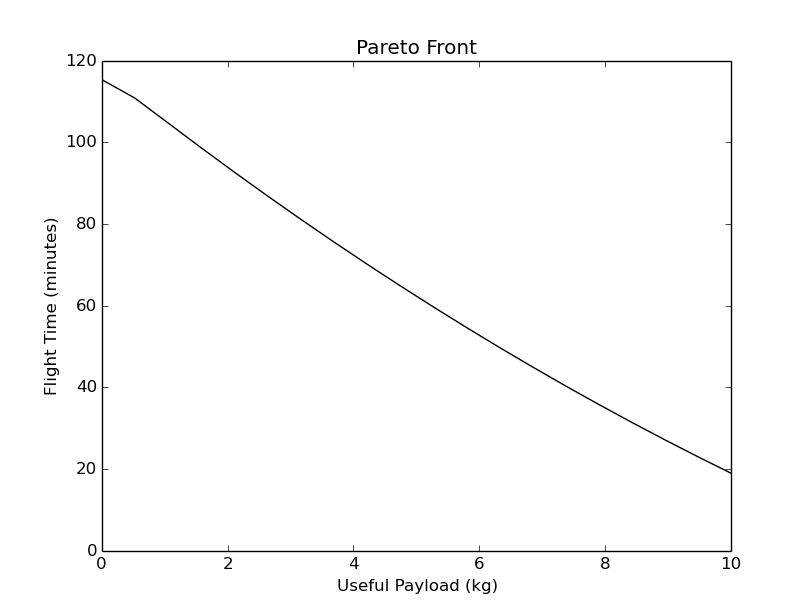
\includegraphics[width=0.5\textwidth]{pareto_front.png}
	\caption{Pareto fronter like curve found by optimizing for flight time given specified payloads.}
		\label{fig:payload}
\end{figure}

\begin{figure}
	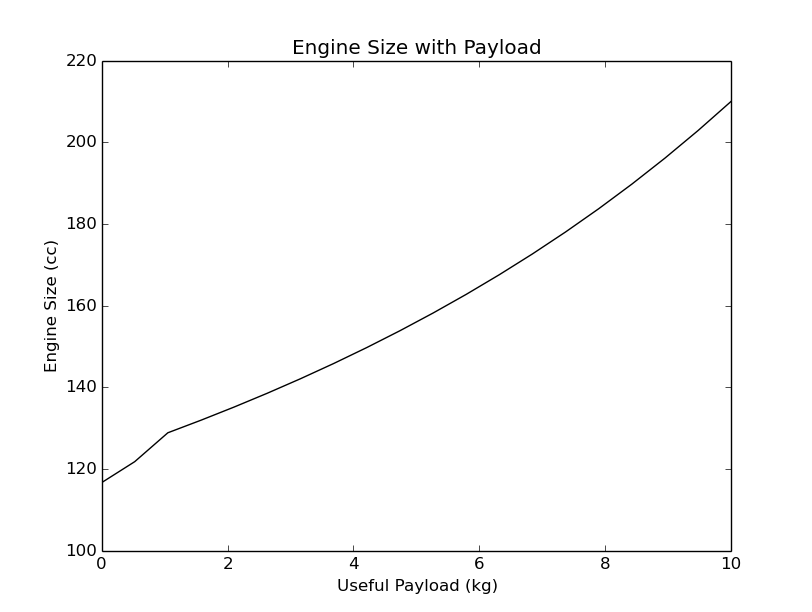
\includegraphics[width=0.5\textwidth]{engine_size_vs_payload.png}
	\caption{Optimal engine size (cc) given a specified payload.}
		\label{fig:eng_v_pl}
\end{figure}

Because the final design requires a single optimal solution and not a range of solutions that depend on our payload capacity we then simultaneously optimize at several payloads. This means the optimization must maximize the total combined flight time while stratifying constraints for operating points.

\section{RESULTS AND DISCUSSION}

When simultaneously optimizing with 3, 5, and 7 kg payloads we get an optimal solution. The solution flight time is at least 42.46 minutes with a payload less then 7 kg. The values of the optimal design variables can be seen in table~\ref{table:unbound_results}. 

\begin{tablehere}
\centering
\vspace{5mm}
	\begin{tabulary}{0.5\textwidth}{|C|C|}
		\hline
		Design Variable & Optimal Value \\ \hline \hline
		Rotor radius (m) & 2.156 \\ \hline
		Engine size (cc) & 176.9 \\ \hline
		Fuel Capacity (kg) & 6.45 \\ \hline
		Fuel burn rate (g/s) & 1.898 \\ \hline
		Rotor pitch (deg) & 17.6 \\ \hline
		Head speed (rpm) & 135.1 \\ \hline
	\end{tabulary}
\caption{Optimal design variables for loosely bound constraints.}
\label{table:unbound_results}
\end{tablehere}

The above solution is a vehicle with an unreasonably large slow moving propellers. While bounding our rotor size would give a more physically manageable solution, it would have also meant our optimization was largely an aerodynamic analysis with a small optimization of engine size. Leaving the variable loosely bounded gives more insight about the trade offs of the vehicle makes for efficiency. 

We also found that the solutions varied greatly with very small changes in our aerodynamic analysis. Personal experience with RC aircraft lead us to believe that the head speed and pitch angles are too extreme. Further validation of our analysis would be required before a design such as this to be built. 


%%%%%%%%%%%%%%%%%%%%%%%%%%%%%%%%%%%%%%%%%%%%%%%%%%%%%%%%%%%%%%%%%%%%%%%%%%%%%%%%%%

\section{CONCLUSION}

lots of really good conclusions

%%%%%%%%%%%%%%%%%%%%%%%%%%%%%%%%%%%%%%%%%%%%%%%%%%%%%%%%%%%%%%%%%%%%%%%%%%%%%%%%
% \section*{APPENDIX}

% Appendixes should appear before the acknowledgment.

% \section*{ACKNOWLEDGMENT}

% Important people/organizations who made it possible


%%%%%%%%%%%%%%%%%%%%%%%%%%%%%%%%%%%%%%%%%%%%%%%%%%%%%%%%%%%%%%%%%%%%%%%%%%%%%%%%

\bibliography{./library}
\bibliographystyle{ieeetr}



\end{document}


%%%%%%%%%%%%%%%%%%%%%%%%%%%%%%%%%%%%%%%%%%%%%%%%%%%%%%%%%%%%%%%%%%%%%%%%%%%%%

% SAVED STUFF






%new document




